\documentclass[11pt,a4paper]{article}
\usepackage[margin=2cm]{geometry}
\usepackage{amsmath,amssymb,bm}
\usepackage{booktabs}
\usepackage{graphicx}
\usepackage{xcolor}
\usepackage{algorithm}
\usepackage{algpseudocode}
\usepackage{caption}
\usepackage{subcaption}
\usepackage{enumitem}
\usepackage{float}
\usepackage{placeins}
\usepackage{microtype}
\usepackage[hidelinks]{hyperref}
\usepackage{setspace}
\setstretch{1.05}
\graphicspath{{../figures/}}
\captionsetup{font=small,labelfont=bf,skip=6pt}
\captionsetup[sub]{font=small,skip=2pt}

\title{%
  Numerical Solution of a Variable-Diffusion Elliptic BVP\\[0.4em]
  \large Project 2 (PDE BVP) Report --- Team 15
}
\author{Chuyang Wang, 2363591 \quad (solo)\\[0.3em]
Department of Applied Mathematics}
\date{October 2026}

\begin{document}
\maketitle

\begin{abstract}
Steady heat conduction in a heterogeneous medium is modelled by the divergence-form elliptic problem
\(-\nabla\cdot(a\nabla u)=f\) on the unit square (Problem Pack Direction~3).
I discretise with a conservative face-averaged five-point finite-difference scheme, assemble in COO, solve in CSR, and move Dirichlet data into the right-hand side so that boundary nodes are never unknowns.
On the smooth manufactured benchmark \(a=1+x\), \(u^*=\sin(\pi x)\sin(\pi y)\), discrete \(L^2\) and \(L^\infty\) errors both fit order \(2.00\) over \(n=15,31,63,127\), with \(\|A-A^\top\|_{\max}/\|A\|_{\max}=0\).
On the layered jump \(a=1\,|\,10\) at \(x=1/2\), a harmonic face average is nodally exact (\(L^\infty\sim 10^{-14}\)) and recovers the interface flux \(20/11\); the arithmetic average of the same nodal values yields first-order \(L^\infty\) error and an \(\mathcal{O}(1)\) flux jump under refinement.
Unpreconditioned CG matches the direct discrete \(L^2\) error once the relative residual reaches \(10^{-4}\); at \(n=31\) there is no runtime crossover with \texttt{spsolve}.
The scheme is second-order for smooth \(a\); across an unresolved jump an arithmetic face coefficient loses both order and flux continuity, and CG iteration counts grow with contrast \(a_R/a_L\).
\end{abstract}

\noindent\textbf{Keywords:} elliptic BVP, variable diffusion, five-point stencil, harmonic average, method of manufactured solutions, sparse direct / CG

\tableofcontents
\newpage

\section{Introduction and Motivation}
\subsection{Problem Background}
Steady heat conduction in a layered composite, soil profile, or tissue boundary is the model problem in which the conductivity \(a(x,y)\) varies in space and may jump~\cite{problemPack,hackbusch2017}.
The physically correct operator is the divergence form \(-\nabla\cdot(a\nabla u)\): the normal flux \(a\partial_n u\) is continuous across an interface.
A pointwise expansion \(a\Delta u+\nabla a\cdot\nabla u\) is the wrong starting point once \(a\) is discontinuous---it loses conservation, symmetry, and the M-matrix sign pattern.

I chose Direction~3 rather than a curved-disk Poisson problem because the unit square keeps the five-point machinery of Tutorial~5 intact, while the jump forces a modelling choice (arithmetic versus harmonic face coefficients) that a smooth manufactured Poisson problem never sees.
This is a solo submission: stencil, solvers, experiments, and text are mine.

\subsection{Mathematical Model}
On \(\Omega=(0,1)^2\) with Dirichlet data on \(\partial\Omega=\Gamma_D\),
\begin{equation}
-\nabla\cdot\bigl(a(x,y)\nabla u\bigr)=f\quad\text{in }\Omega,\qquad
u=g\quad\text{on }\partial\Omega,
\label{eq:pde}
\end{equation}
with \(0<a_{\min}\le a(x,y)\le a_{\max}<\infty\).
The sign convention makes \(-\nabla\cdot(a\nabla u)\) a positive operator, so the discrete matrix has a positive diagonal.
There is no Neumann part: \(\Gamma_N=\emptyset\).

\paragraph{Smooth manufactured benchmark (bank P4).}
\[
a(x,y)=1+x,\qquad
u^*(x,y)=\sin(\pi x)\sin(\pi y),\qquad
g=0,
\]
and
\begin{equation}
f=2\pi^2(1+x)\sin(\pi x)\sin(\pi y)-\pi\cos(\pi x)\sin(\pi y).
\label{eq:f4}
\end{equation}
The extra \(-\pi\cos(\pi x)\sin(\pi y)\) term is \(\nabla a\cdot\nabla u^*\); a constant-coefficient five-point stencil cannot capture it.

\paragraph{Layered-interface benchmark.}
\[
a(x)=\begin{cases}1,&x<1/2,\\10,&x>1/2,\end{cases}
\qquad f=0,
\]
and \(g=u^*\) on \(\partial\Omega\), where the exact one-dimensional profile
\begin{equation}
u^*(x)=\begin{cases}
\dfrac{20}{11}\,x,&0\le x\le 1/2,\\[4pt]
\dfrac{2}{11}\,x+\dfrac{9}{11},&1/2\le x\le 1,
\end{cases}
\label{eq:ulayered}
\end{equation}
is independent of \(y\).
It is continuous, \(u^*(0)=0\), \(u^*(1)=1\), the derivative jumps, and the flux \(a u_x^*=20/11\) is continuous.
Well-posedness follows from uniform ellipticity and a nonempty Dirichlet boundary; no compatibility condition is required.

Expected signs: on the layered problem, \(u^*\in[0,1]\) with extrema on the boundary (maximum principle).
On P4, \(u^*>0\) in \(\Omega\) and \(u^*=0\) on \(\partial\Omega\).

\subsection{Overview of the Report}
Section~\ref{sec:disc} derives the face-averaged stencil and Dirichlet shift, states truncation assumptions, and links energy stability to convergence---including the series-resistance derivation of the harmonic face mean.
Section~\ref{sec:impl} records the implementation.
Section~\ref{sec:exp} verifies P4 by MMS, separates algebraic from discretisation error, falsifies ``symmetry \(\Rightarrow\) correct interface,'' and reports cost at a matched accuracy target.
Section~\ref{sec:conc} summarises the findings.

\section{Discretisation and Analysis}
\label{sec:disc}
\subsection{Discrete Scheme}
I use a uniform nodal grid with \(n\) interior nodes per direction,
\begin{equation}
h=\frac{1}{n+1},\qquad
x_i=(i+1)h,\qquad
y_j=(j+1)h,\qquad
i,j=0,\ldots,n-1.
\label{eq:grid}
\end{equation}
The unknown vector is indexed by \(k=i n+j\) (\texttt{meshgrid} with \texttt{indexing='ij'}; axis \(0\) is \(x\)).
Boundary nodes are not unknowns.

A conservative finite-volume reading of \(-\nabla\cdot(a\nabla u)\) on the dual cell of width \(h\) gives the five-point divergence-form stencil~\cite{leveque2007,problemPack}
\begin{equation}
(A_h U)_{ij}
=\frac{1}{h^2}\Bigl[
a_E(U_{ij}-U_{i+1,j})
+a_W(U_{ij}-U_{i-1,j})
+a_N(U_{ij}-U_{i,j+1})
+a_S(U_{ij}-U_{i,j-1})
\Bigr].
\label{eq:stencil}
\end{equation}
When \(a\equiv 1\) this recovers the classical five-point Laplacian
\[
(-\Delta_h u)_{ij}=\frac{4u_{ij}-u_W-u_E-u_S-u_N}{h^2}.
\]
The four face coefficients are shared: the east coefficient of node \((i,j)\) is the west coefficient of node \((i+1,j)\).
That sharing makes \(A_h\) symmetric after Dirichlet elimination.

For smooth \(a\) I evaluate the coefficient at the half-point, \(a_E=a(x_i+h/2,y_j)\).
For \(a=1+x\) this coincides with the arithmetic nodal midpoint and is second-order.
At a material interface I use the resistance (harmonic) average of the two nodal values,
\begin{equation}
a_E=\frac{2 a_L a_R}{a_L+a_R},
\label{eq:harm}
\end{equation}
and, as the depth comparison, the arithmetic mean \((a_L+a_R)/2\).
When the interface bisects a grid edge, \eqref{eq:harm} is exact for piecewise-constant \(a\).
I therefore take odd interval counts \(N=n+1\in\{31,63,127,255\}\) on the layered test, so \(x=1/2\) lies midway between two interior columns~\cite{problemPack}.

\subsection{Consistency and Truncation Error}
For a single east face with smooth \(a\) and \(u\), the centred flux
\[
a_E\frac{U_{i+1,j}-U_{ij}}{h}
=
a\!\left(x_i+\tfrac{h}{2},y_j\right)\,u_x\!\left(x_i+\tfrac{h}{2},y_j\right)
+\mathcal{O}(h^2)
\]
is second-order; summing four such faces and dividing by \(h\) recovers \(-\nabla\cdot(a\nabla u)+\mathcal{O}(h^2)\).
The same \(u_{xxxx}\) and \(u_{yyyy}\) pieces appear as in the five-point Laplacian, plus smooth lower-order terms from \(\nabla a\).
Assumptions: \(u\in C^4(\overline{\Omega})\) and \(a\in C^2(\overline{\Omega})\).
Across the layered jump, \(u^*\) is only Lipschitz and \(a\notin C^2\), so this expansion fails at the interface face; second-order truncation is not claimed for an arithmetic coefficient there.

I measure the truncation residual \(\tau_h=b-A_h u^*\) in the discrete \(L^2\) norm \(h\|\tau_h\|_2\).
On P4 this quantity drops by four under each mesh doubling (Table~\ref{tab:trunc}), consistent with \(\mathcal{O}(h^2)\) pointwise truncation.
On the four meshes of Table~\ref{tab:p4} there is no finest-mesh floor: both named errors continue to quarter, so the fitted order \(2.00\) is not contaminated by round-off.

\subsection{Boundary Treatment}
Every neighbour that lands on \(\partial\Omega\) is removed from the unknown list.
If the stencil at interior index \(k\) has a Dirichlet neighbour with value \(g_{\mathrm{edge}}\), the term \(a_{\mathrm{face}}(U_k-g_{\mathrm{edge}})/h^2\) contributes
\begin{equation}
b_k \mathrel{+}= \frac{a_{\mathrm{face}}\,g_{\mathrm{edge}}}{h^2}
\label{eq:dirichlet}
\end{equation}
to the right-hand side.
For P5 (\(u^*=e^x\sin(\pi y)\), \(a=1\)) the west column \(i=0\) is the row set \(k=0,\ldots,n-1\); an example is
\[
b[0]\mathrel{+}=\frac{e^{0}\sin(\pi y_0)}{h^2}.
\]
Replacing a Dirichlet row by \(e_k\) while leaving the corresponding column untouched would destroy symmetry~\cite{problemPack}.
Boundary nodes are therefore absent from \(A_h\).
All boundaries are Dirichlet; there is no Neumann/Robin closure.

\subsection{Discrete Structure, Stability, and Convergence}
After Dirichlet elimination, every off-diagonal entry of \(A_h\) is non-positive and the row sums on interior stencils that do not touch the boundary are zero; boundary-adjacent rows are strictly diagonally dominant because a positive \(a_{\mathrm{face}}/h^2\) has been moved to \(b\).
With positive shared face coefficients, \(A_h\) is a symmetric M-matrix, hence SPD, and the discrete maximum principle holds: a discrete solution of \(A_h U=0\) with Dirichlet data in \([m,M]\) remains in \([m,M]\).

This is stability for the present coefficients and BCs, not a generic periodic von~Neumann argument.
The continuous energy identity for~\eqref{eq:pde} with homogeneous Dirichlet data is
\begin{equation}
\int_\Omega a|\nabla u|^2\,\mathrm{d}x
=\int_\Omega f u\,\mathrm{d}x,
\label{eq:energy}
\end{equation}
so coercivity is controlled by \(a_{\min}>0\).
On the grid, the shared-face assembly is the discrete analogue: \(U^\top A_h U=\sum_{\mathrm{faces}} a_{\mathrm{face}}(\delta U)^2/h^2\ge a_{\min}\,|U|_{H^1_h}^2\).
Dirichlet elimination does not destroy that identity because boundary values enter \(b\), not the quadratic form on interior unknowns.
Consequently \(A_h\) remains SPD for every admissible \(a\) used in this report (smooth \(a=1+x\) and both harmonic/arithmetic layered averages).

\paragraph{Why the harmonic mean is forced at a jump.}
Across a vertical interface the exact flux \(q=a u_x\) is continuous.
On one grid edge of length \(h\) that straddles \(a_L\) and \(a_R\) in equal halves, integrating \(u_x=q/a\) gives
\begin{equation}
U_R-U_L
=q\cdot\tfrac{h}{2}\Bigl(\tfrac{1}{a_L}+\tfrac{1}{a_R}\Bigr)
\quad\Rightarrow\quad
q=\frac{2 a_L a_R}{a_L+a_R}\,\frac{U_R-U_L}{h}.
\label{eq:series}
\end{equation}
So the face coefficient that preserves the continuous flux is exactly~\eqref{eq:harm}.
The arithmetic mean \((a_L+a_R)/2\) is a different resistance and cannot match \(q\) unless \(a_L=a_R\).
This is a transmission identity for Direction~3, not a quoted textbook stencil for \(-\Delta\).

\paragraph{Convergence.}
On smooth data, consistency of order \(2\) plus the M-matrix / energy stability above imply convergence of order \(2\) in the discrete \(L^2\) and \(L^\infty\) norms (Lax equivalence for linear FD schemes).
Table~\ref{tab:p4} confirms the rate numerically: fitted slopes \(2.00\) with no deviation on the four meshes.
On the layered jump the regularity assumption fails, so the theorem does not apply: harmonic averaging restores nodal exactness via~\eqref{eq:series}, while arithmetic averaging drops to first order (Table~\ref{tab:layer})---the observed deviation from order \(2\) is therefore predicted, not anomalous.

Three numerical checks corroborate the derivation:
\(\|A-A^\top\|_{\max}/\|A\|_{\max}=0\) on every assembled matrix in this report;
the smallest algebraic eigenvalue of the P4 matrix at \(n=15\) is \(\lambda_{\min}=28.61>0\);
the layered numerical solution stays in \([0,1]\).
Conditioning is separate: \(\kappa_2(A_h)\) on P4 grows like \(h^{-2}\) (\(126.5\), \(529.7\), \(2.18\times 10^3\) at \(n=15,31,63\)), as expected for a second-order elliptic operator.

\section{Implementation}
\label{sec:impl}
\subsection{Algorithm}
\begin{algorithm}[H]
\caption{Assembly of \(A_h U=b\) and the direct solve}
\begin{algorithmic}[1]
\Require interior count \(n\), coefficient \(a\), data \(f,g\), face rule (half-point / harmonic / arithmetic)
\Ensure \(u_h\), residual \(\|b-A_h u_h\|_\infty\)
\State \(h\leftarrow 1/(n+1)\); index \(k=in+j\)
\State \(b\leftarrow f\) sampled at interior nodes
\For{each interior node \((i,j)\)}
  \For{each of the four faces}
    \State compute a shared \(a_{\mathrm{face}}>0\)
    \If{the neighbour is interior}
      \State add \(a_{\mathrm{face}}/h^2\) to the diagonal and \(-a_{\mathrm{face}}/h^2\) to that column
    \Else
      \State add \(a_{\mathrm{face}}/h^2\) to the diagonal and \(a_{\mathrm{face}} g_{\mathrm{edge}}/h^2\) to \(b_k\)
    \EndIf
  \EndFor
\EndFor
\State convert COO triplets to CSR; \(u_h\leftarrow\texttt{spsolve}(A,b)\)
\State report \(\|b-A u_h\|_\infty\)
\end{algorithmic}
\end{algorithm}
\noindent
Lines 4--11 build one shared face at a time so that \(A_h\) inherits symmetry from the continuous flux form; the Dirichlet branch (lines 9--10) is exactly~\eqref{eq:dirichlet}.
The CSR conversion and \texttt{spsolve} call are the only dense-library steps; assembly itself never materialises a dense \(n^2\times n^2\) array.

\subsection{Code Structure}
\begin{center}
\begin{tabular}{@{}lp{0.72\textwidth}@{}}
\toprule
File & Purpose\\
\midrule
\texttt{model.py} & \(a(x,y)\), manufactured \(u^*\), layered exact profile~\eqref{eq:ulayered}\\
\texttt{assemble.py} & sparse face-averaged stencil, index map, interface flux\\
\texttt{solvers.py} & \texttt{spsolve}, residual-stopped CG, \(\lambda_{\min}\) / \(\kappa\) via \texttt{eigsh}\\
\texttt{verify.py} & named-norm errors, four-mesh tables, layered diagnostics\\
\texttt{plots.py} & every report figure\\
\texttt{fem1d.py} / \texttt{fem2d\_oracle.py} & independent 1D P1 and optional 2D P1 oracles\\
\texttt{test\_problem\_bank.py} & analytic bank (P1--P5), self-check of \(f=-\nabla\cdot(a\nabla u^*)\)\\
\texttt{validation\_tests.py} & sign, boundary, order, nodal-exact, and M-matrix checks\\
\texttt{run\_all.py} & regenerates every figure and prints the quoted numbers\\
\bottomrule
\end{tabular}
\end{center}

\subsection{Key Design Decisions}
I assemble in COO and convert to CSR once.
The physics (\(a\), \(f\), \(g\)) lives in \texttt{model.py}, so the same assembler runs P4, P5 and the layered jump.
The default solve is sparse direct: at the meshes in this report (\(n\le 254\), \(N_{\mathrm{unk}}\le 6.5\times 10^4\), five nonzeros per row) a banded factorisation is cheaper than unpreconditioned CG, which I still run as a residual-stopped iterative check and as a contrast-sensitivity probe.
Cost measure (named before it is quoted): for CG, iteration count to a stated relative residual; for the direct solver, one sparse factorisation, with wall time only as a secondary observation.
I do not count assembly, eigenvalue estimates, or plotting.

\section{Verification and Numerical Experiments}
\label{sec:exp}
\subsection{Verification: Method of Manufactured Solutions}
The bank's finite-difference self-check on \(f=-\nabla\cdot(a\nabla u^*)\) passes with worst relative error \(5.8\times 10^{-6}\) (analytic data check, not a solver test)~\cite{problemPack}.
Sign and boundary gates come first: P2 (\(u^*=x^2-y^2\)) has \(L^\infty=3.3\times 10^{-16}\) at \(n=15\) (exact on this quadratic); P5 recovers the Tutorial~5 centre \(u_h(0.5,0.5)=1.652\).

Table~\ref{tab:p4} is the P4 refinement study.
Named norms: discrete \(L^2\) given by \(h\|u_h-u^*\|_2\), and \(\|u_h-u^*\|_\infty\).
Both fitted log-log slopes on \(n=15,31,63,127\) are \(2.00\) (standard error of the fit \(<10^{-3}\)).
Figure~\ref{fig:order} plots that table; Figure~\ref{fig:field} shows the field and mesh; Figure~\ref{fig:spy} shows the sparsity pattern after elimination.

\begin{table}[H]
\centering
\caption{P4 smooth manufactured solution, face coefficient at the half-point, \texttt{spsolve}. Discrete \(L^2\) means \(h\|u_h-u^*\|_2\).}
\label{tab:p4}
\begin{tabular}{@{}rcccccc@{}}
\toprule
\(n\) & \(h\) & \(L^2\) & \(L^\infty\) & \(\|b-Au_h\|_\infty\) & \(p_{L^2}\) & \(p_\infty\)\\
\midrule
15  & \(1/16\)  & \(1.598\times 10^{-3}\) & \(3.205\times 10^{-3}\) & \(4.48\times 10^{-13}\) & --- & ---\\
31  & \(1/32\)  & \(3.988\times 10^{-4}\) & \(8.009\times 10^{-4}\) & \(3.00\times 10^{-12}\) & \(2.00\) & \(2.00\)\\
63  & \(1/64\)  & \(9.966\times 10^{-5}\) & \(2.003\times 10^{-4}\) & \(1.40\times 10^{-11}\) & \(2.00\) & \(2.00\)\\
127 & \(1/128\) & \(2.491\times 10^{-5}\) & \(5.007\times 10^{-5}\) & \(6.92\times 10^{-11}\) & \(2.00\) & \(2.00\)\\
\bottomrule
\end{tabular}
\end{table}

\begin{table}[H]
\centering
\caption{P4 truncation \(h\|b-A_h u^*\|_2\). Each refinement halves \(h\) and multiplies the truncation by \(\approx 1/4\).}
\label{tab:trunc}
\begin{tabular}{@{}rccc@{}}
\toprule
\(n\) & \(h\) & \(h\|\tau_h\|_2\) & \(\|\tau_h\|_\infty\)\\
\midrule
15  & \(1/16\)  & \(4.978\times 10^{-2}\) & \(1.028\times 10^{-1}\)\\
31  & \(1/32\)  & \(1.248\times 10^{-2}\) & \(2.572\times 10^{-2}\)\\
63  & \(1/64\)  & \(3.122\times 10^{-3}\) & \(6.433\times 10^{-3}\)\\
127 & \(1/128\) & \(7.808\times 10^{-4}\) & \(1.609\times 10^{-3}\)\\
\bottomrule
\end{tabular}
\end{table}

\begin{figure}[H]
\centering
\begin{subfigure}[t]{0.48\textwidth}
  \centering
  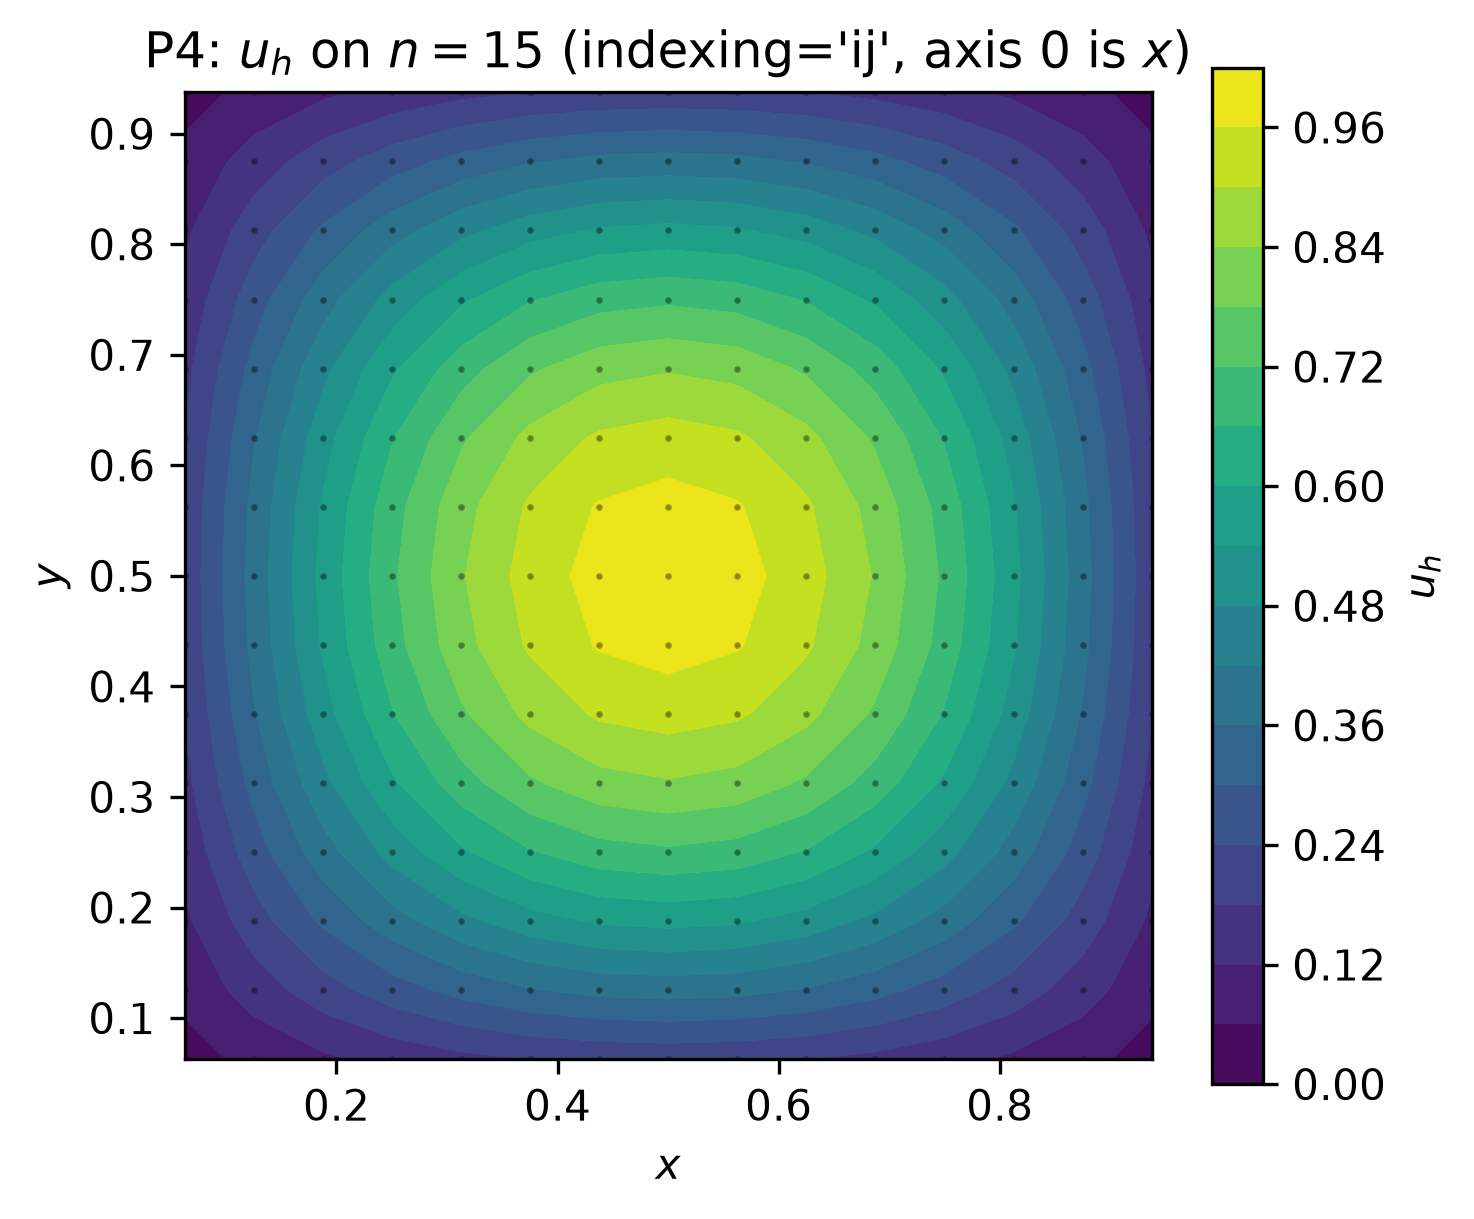
\includegraphics[width=\linewidth]{fig01_smooth_contour.png}
  \caption{Filled contours with interior nodes (\(n=15\)).}
\end{subfigure}\hfill
\begin{subfigure}[t]{0.48\textwidth}
  \centering
  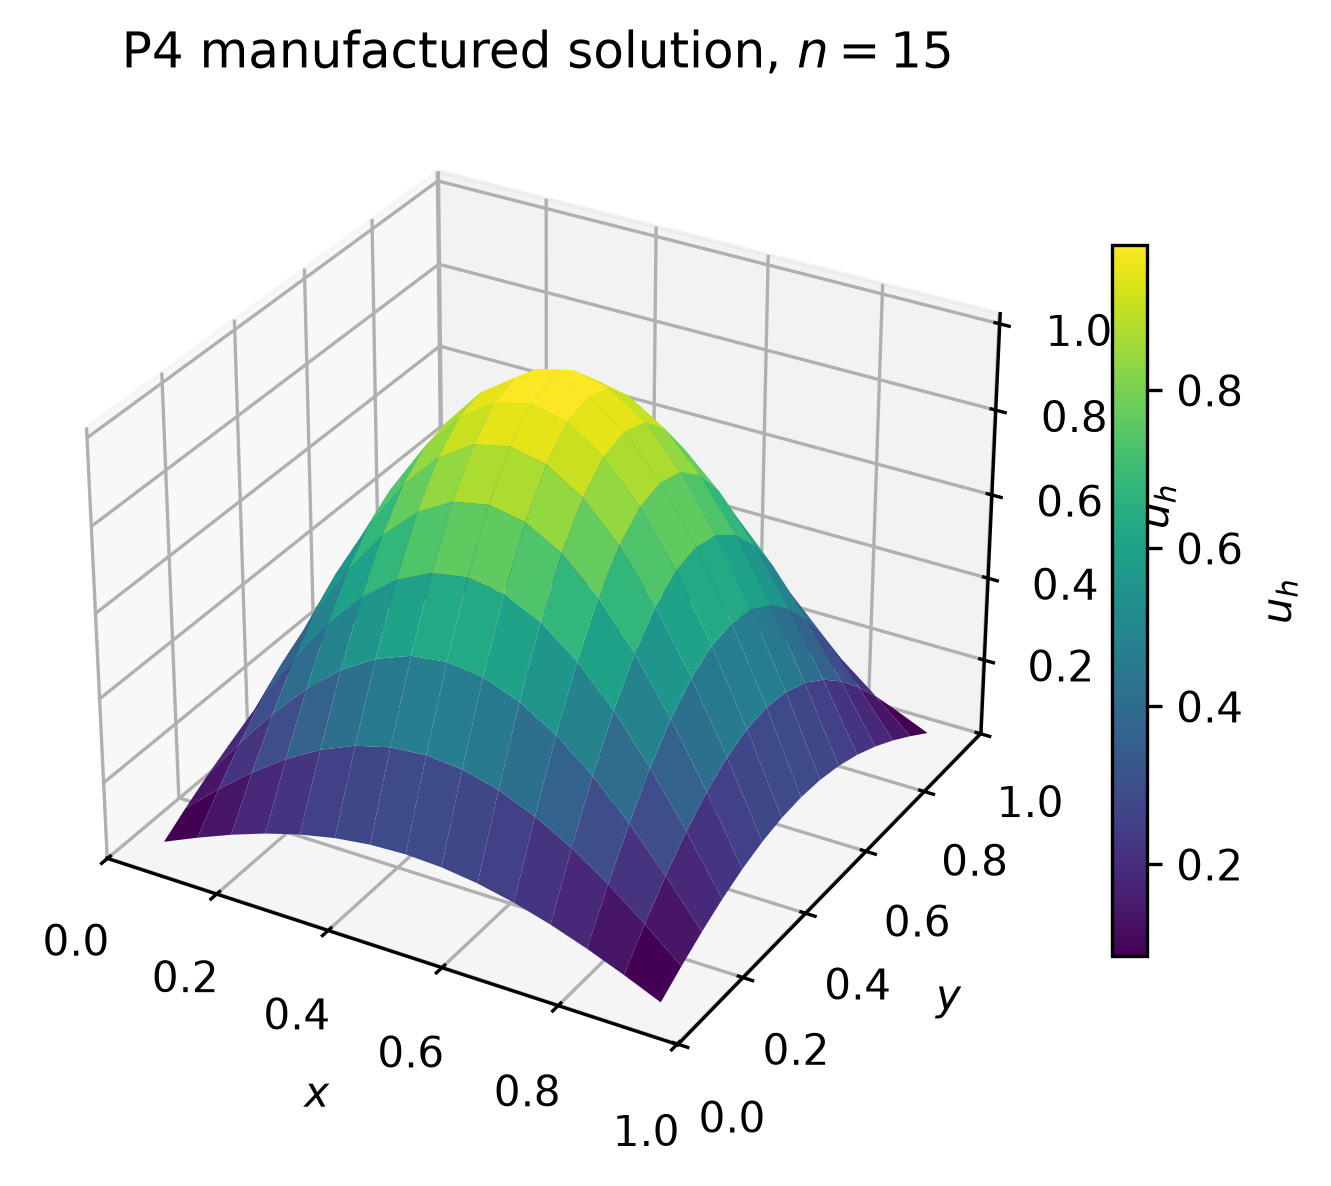
\includegraphics[width=\linewidth]{fig02_smooth_surface.png}
  \caption{Surface plot of \(u_h\).}
\end{subfigure}
\caption{P4 solution at \(n=15\). Mesh convention: \texttt{indexing='ij'}, axis \(0\) is \(x\). Contours show the field the mesh actually resolved.}
\label{fig:field}
\end{figure}

\begin{figure}[H]
\centering
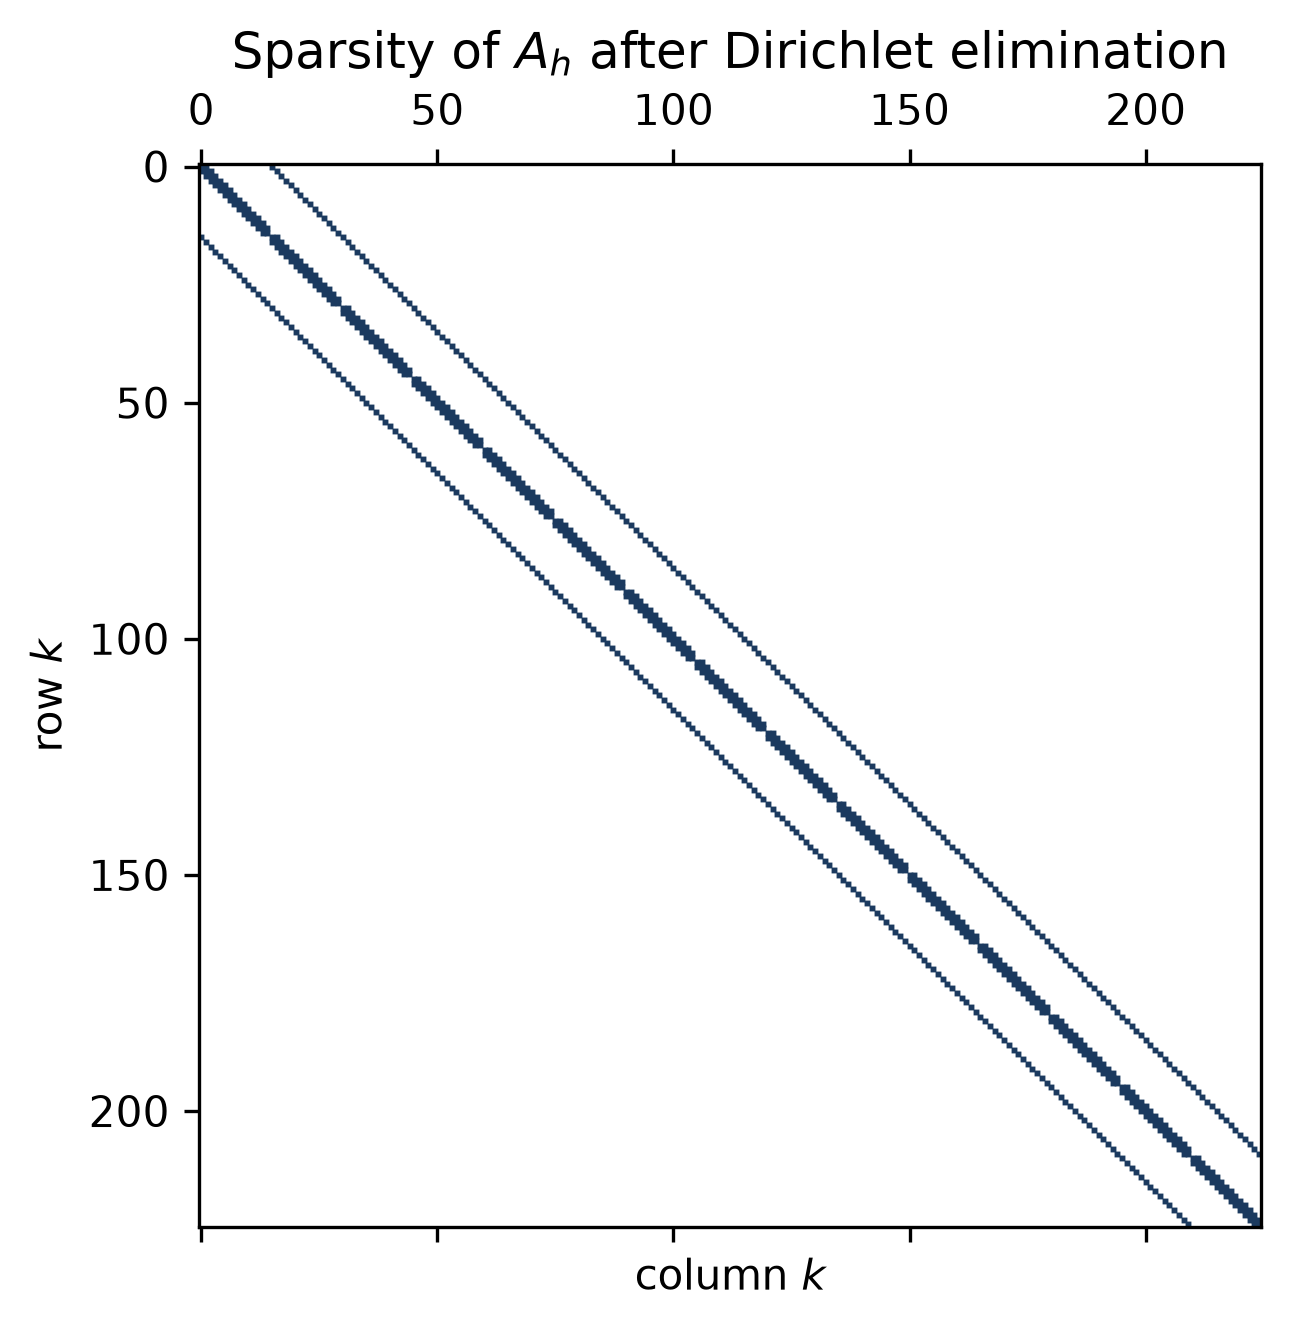
\includegraphics[width=0.42\textwidth]{fig03_spy.png}
\caption{Spy plot of \(A_h\) at \(n=15\) after Dirichlet elimination (\(225\times 225\)). Five-point bandwidth matches the index map \(k=in+j\).}
\label{fig:spy}
\end{figure}

\begin{figure}[H]
\centering
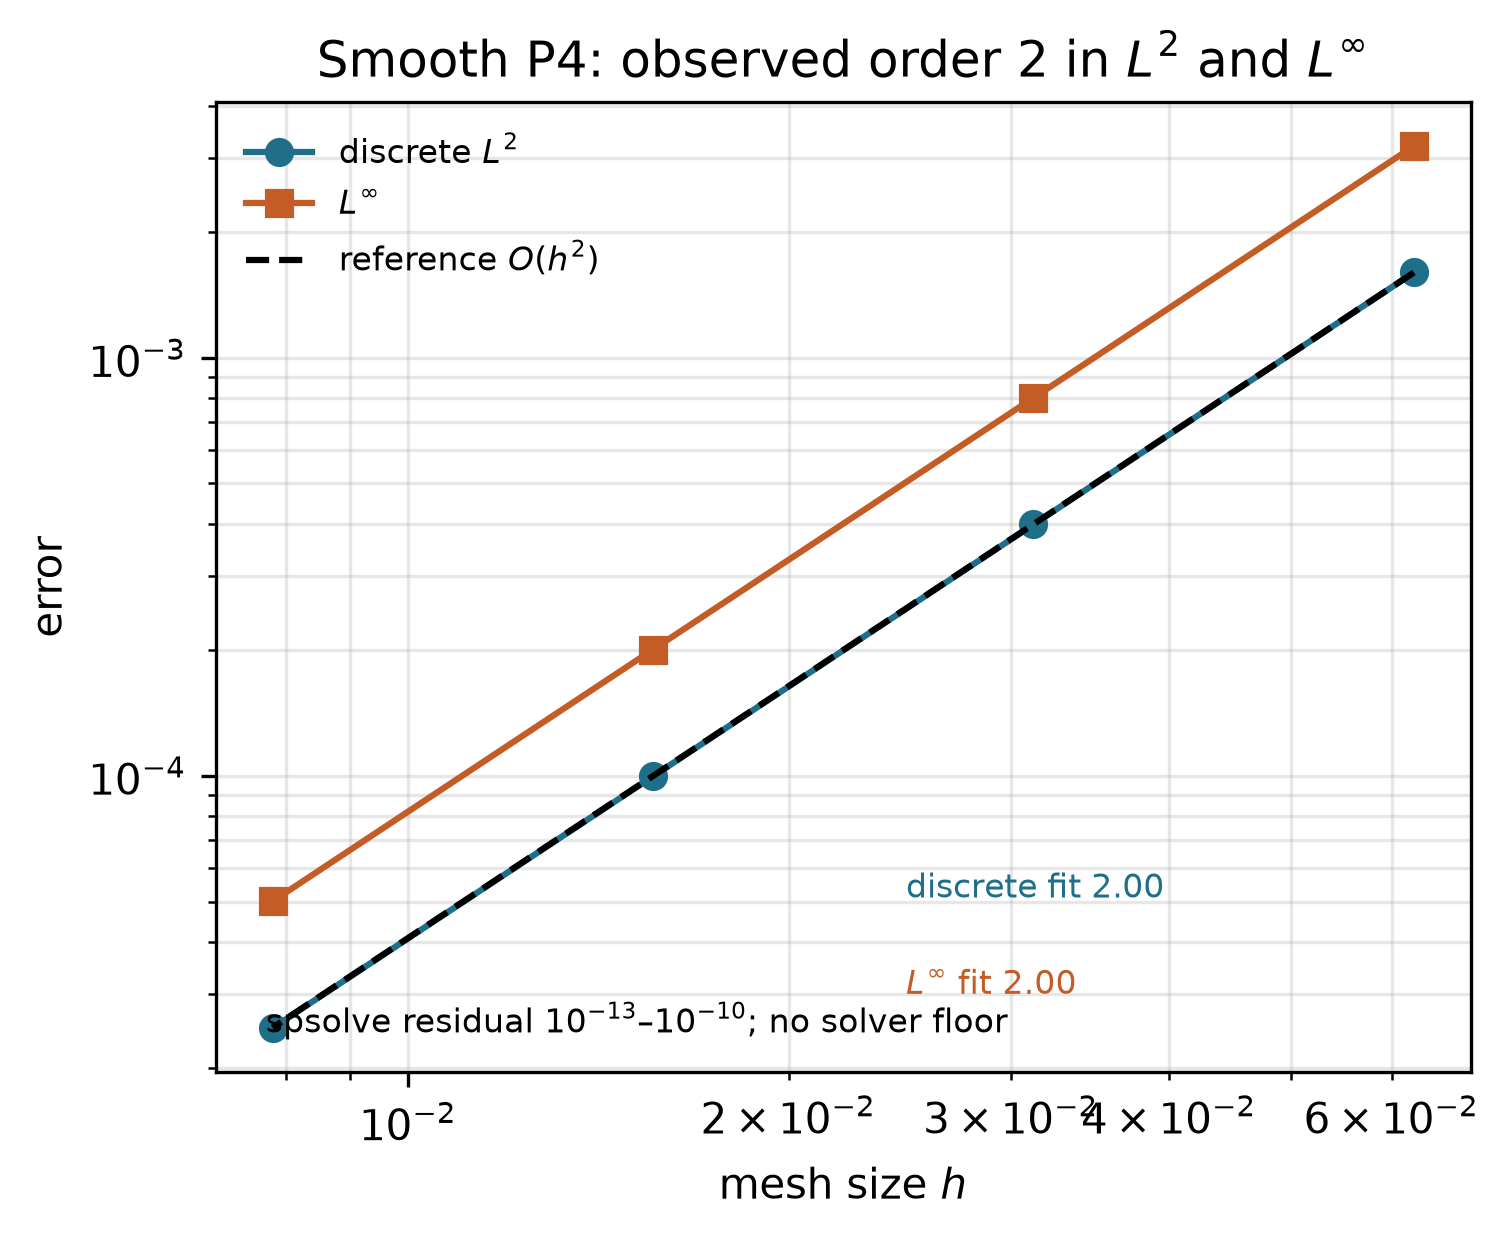
\includegraphics[width=0.62\textwidth]{fig04_order_smooth.png}
\caption{Log-log P4 errors versus \(h\). Fitted discrete-\(L^2\) order \(2.001\pm 0.000\), \(L^\infty\) order \(2.000\pm 0.000\), four meshes, reference slope \(2\). Confirms that the face-averaged stencil is second order on smooth data.}
\label{fig:order}
\end{figure}

An independent 2D P1 FEM solve of the same P4 data (\texttt{scikit-fem}, homogeneous Dirichlet by \texttt{condense}) gives \(L^2=5.18\times 10^{-3}\) at \(h_{\max}=8.84\times 10^{-2}\), residual \(2\times 10^{-15}\): an order-of-magnitude cross-check on a different mesh and method.
The 1D P1 training problem \(-\,u''=\pi^2\sin(\pi x)\) with nodal trapezoidal load fits discrete-\(L^2\) order \(2.00\); the hand-checked element matrix is
\[
K^{(e)}=\frac{1}{h}\begin{pmatrix}1&-1\\-1&1\end{pmatrix},\qquad
h=\tfrac14 \;\Rightarrow\;
\begin{pmatrix}4&-4\\-4&4\end{pmatrix}.
\]

\subsection{Separating Algebraic and Discretisation Error}
\texttt{spsolve} has no tolerance parameter.
I treat its solution as the exact discrete solution and report the backward residual.
On P4 at \(n=31\), \(\|b-Au_h\|_\infty=3.00\times 10^{-12}\) while the discrete \(L^2\) error is \(3.99\times 10^{-4}\).
A crude forward-error sketch \(\|e\|_2\lesssim \|r\|_2/\lambda_{\min}\) with \(\lambda_{\min}\approx 28.7\) puts the algebraic error near \(10^{-13}\), four orders below the discretisation error.

Unpreconditioned CG on the same matrix, stopped on the relative residual \(\|r_k\|_\infty/\|r_0\|_\infty\), is the second demonstration (Figure~\ref{fig:cg}).
At relative tolerance \(10^{-2}\) the discrete \(L^2\) error is still \(4.33\times 10^{-4}\); from \(10^{-4}\) onwards it has locked onto the direct value \(3.988\times 10^{-4}\) (Table~\ref{tab:cg}).
Tightening further does not change the reported discretisation error, so the fitted order in Table~\ref{tab:p4} is the discretisation rate.
I stop CG on the residual, never on \(\|x^{k+1}-x^k\|\).

\begin{table}[H]
\centering
\caption{P4, \(n=31\): CG versus \texttt{spsolve}. Cost for CG is iteration count; \texttt{spsolve} is one factorisation (\(0.002\,\mathrm{s}\) wall). The \(L^2\) column is the quantity of interest.}
\label{tab:cg}
\begin{tabular}{@{}lccc@{}}
\toprule
Solve & iterations & \(\|b-Au\|_\infty\) & discrete \(L^2\)\\
\midrule
CG, rel.\ \(10^{-2}\) & 26 & \(7.5\times 10^{-1}\) & \(4.329\times 10^{-4}\)\\
CG, rel.\ \(10^{-4}\) & 39 & \(5.9\times 10^{-3}\) & \(3.988\times 10^{-4}\)\\
CG, rel.\ \(10^{-6}\) & 43 & \(1.3\times 10^{-5}\) & \(3.988\times 10^{-4}\)\\
CG, rel.\ \(10^{-10}\) & 47 & \(3.5\times 10^{-9}\) & \(3.988\times 10^{-4}\)\\
\texttt{spsolve} & --- & \(3.0\times 10^{-12}\) & \(3.988\times 10^{-4}\)\\
\bottomrule
\end{tabular}
\end{table}

\begin{figure}[H]
\centering
\begin{subfigure}[t]{0.48\textwidth}
  \centering
  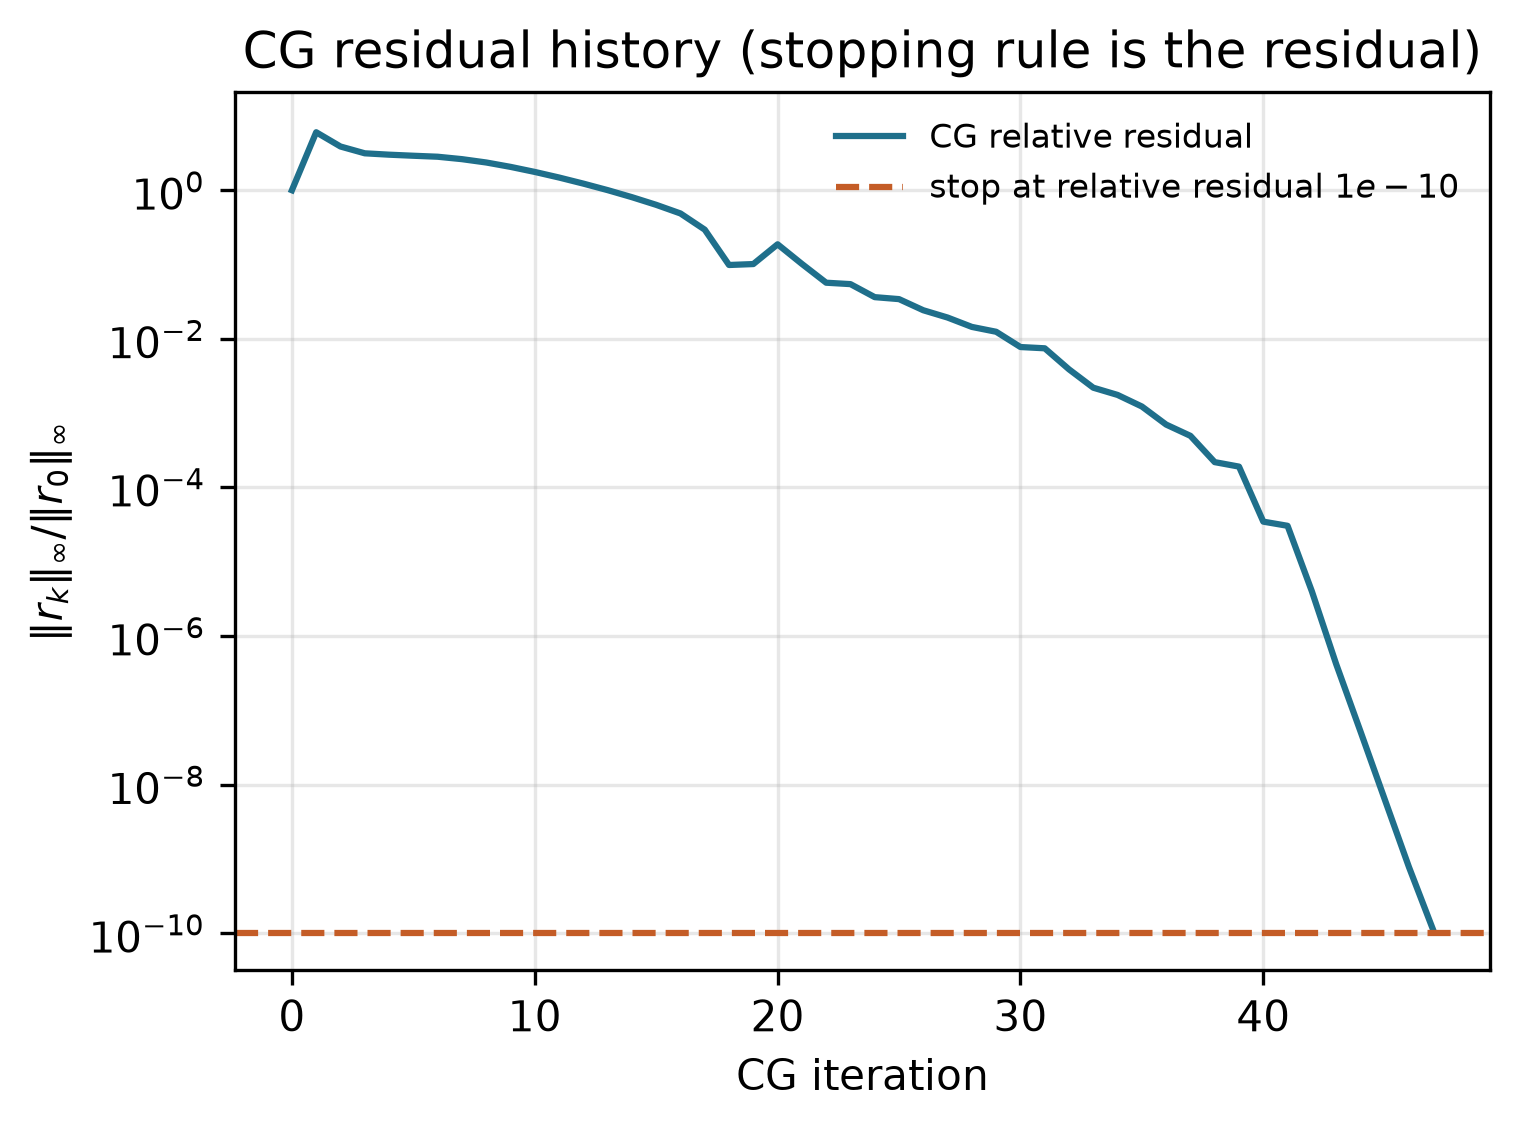
\includegraphics[width=\linewidth]{fig09_cg_residual.png}
  \caption{CG relative residual vs.\ iteration.}
\end{subfigure}\hfill
\begin{subfigure}[t]{0.48\textwidth}
  \centering
  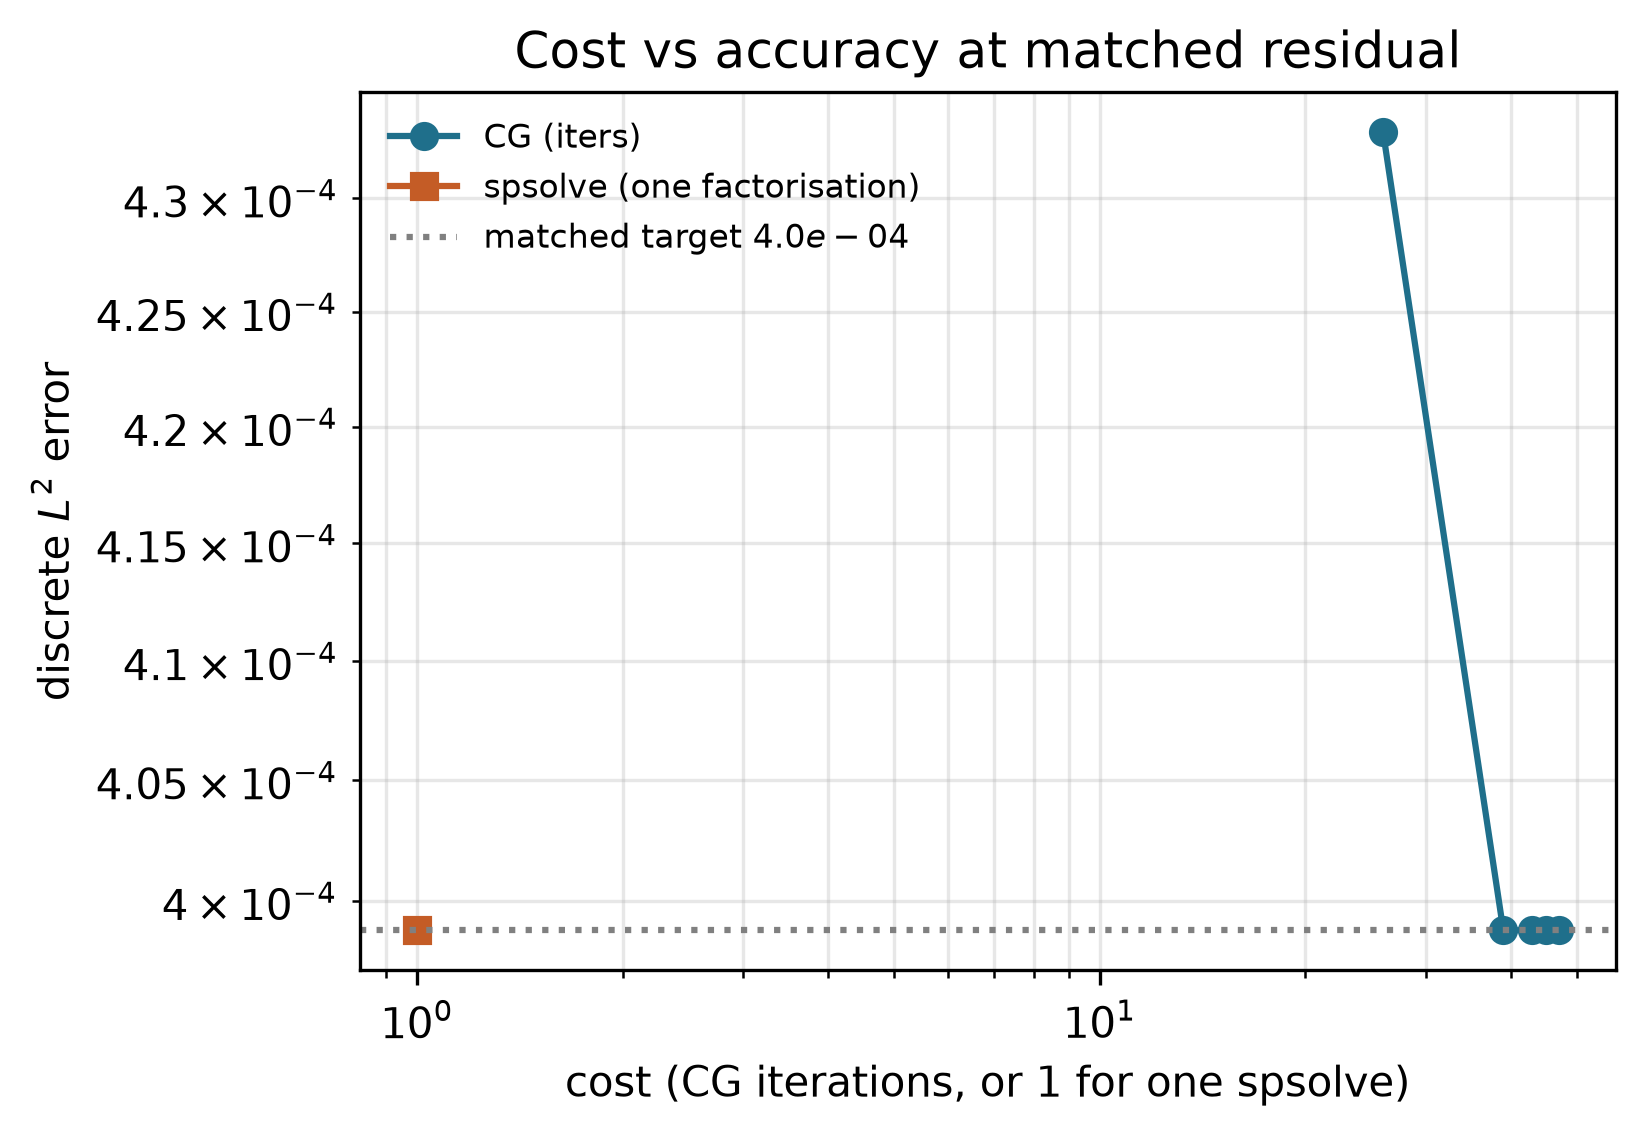
\includegraphics[width=\linewidth]{fig10_cost_accuracy.png}
  \caption{Discrete \(L^2\) vs.\ CG iterations.}
\end{subfigure}
\caption{Left: residual history with stopping line at \(10^{-10}\). Right: discrete \(L^2\) versus CG iterations; dashed line is the \texttt{spsolve} error. Once the residual is tight enough the error floor is discretisation. At \(n=31\) both solves finish in about \(2\,\mathrm{ms}\).}
\label{fig:cg}
\end{figure}

\subsection{Depth Comparison: Harmonic versus Arithmetic Face Coefficients}
This is the project's depth contribution beyond a smooth MMS: the same scheme, same grids, same Dirichlet data~\eqref{eq:ulayered}, same direct solver; only the face rule changes.
The hypothesis under test is that ``any positive face average that keeps \(A_h\) symmetric is an acceptable interface scheme.''
Table~\ref{tab:layer} and Figures~\ref{fig:profile}--\ref{fig:layerorder} falsify that hypothesis and confirm~\eqref{eq:series}.

Harmonic averaging is nodally exact: \(L^\infty\le 3\times 10^{-14}\) on all four meshes, and the numerical flux \(a_E(U_R-U_L)/h\) equals \(20/11\) to at most \(5\times 10^{-13}\) (the pack's sanity check)~\cite{problemPack}.
An interface-fitted 1D P1 FEM with \(32\) elements (so \(x=1/2\) is a node) reproduces the same profile to \(L^\infty=6.7\times 10^{-16}\).
Two methods that share neither the stencil nor the mesh convention agree on the exact nodal values.

Arithmetic averaging still produces a symmetric M-matrix, but the wrong series resistance in~\eqref{eq:series}.
The flux jump stays \(\approx 0.66\) under refinement (\(\mathcal{O}(1)\), not \(\mathcal{O}(h)\)).
The \(L^\infty\) solution error is first-order (\(\approx 1.94\times 10^{-2}\) down to \(2.38\times 10^{-3}\) as \(N\) runs through \(31,63,127,255\)).
Relative to the smooth-case energy~\eqref{eq:energy}, the flux error is the physically meaningful defect: arithmetic keeps a discrete energy form but with the wrong \(a_{\mathrm{face}}\), so \(L^2\)-looking plots can look stable while transport is wrong.

On every harmonic and arithmetic run the discrete solution stays in \([0,1]\): both averages inherit the M-matrix / DMP.
Monotonicity alone does not select the correct face rule.
Value of the comparison: it separates algebraic structure (symmetry, SPD) from interface modelling (flux continuity), which is the core numerical lesson of Direction~3.

\begin{table}[H]
\centering
\caption{Layered \(a=1\,|\,10\), odd interval counts so \(x=1/2\) bisects a grid edge. Flux jump is \(\max_j|a_E(U_R-U_L)/h-20/11|\).}
\label{tab:layer}
\begin{tabular}{@{}rrcccc@{}}
\toprule
\(n\) & \(N\) & harm.\ \(L^\infty\) & harm.\ flux jump & arith.\ \(L^\infty\) & arith.\ flux jump\\
\midrule
30  & 31  & \(3.8\times 10^{-15}\) & \(3.3\times 10^{-14}\) & \(1.94\times 10^{-2}\) & \(0.663\)\\
62  & 63  & \(8.9\times 10^{-15}\) & \(1.3\times 10^{-13}\) & \(9.60\times 10^{-3}\) & \(0.662\)\\
126 & 127 & \(2.5\times 10^{-14}\) & \(1.6\times 10^{-13}\) & \(4.78\times 10^{-3}\) & \(0.662\)\\
254 & 255 & \(2.7\times 10^{-14}\) & \(5.2\times 10^{-13}\) & \(2.38\times 10^{-3}\) & \(0.662\)\\
\bottomrule
\end{tabular}
\end{table}

\begin{figure}[H]
\centering
\begin{subfigure}[t]{0.48\textwidth}
  \centering
  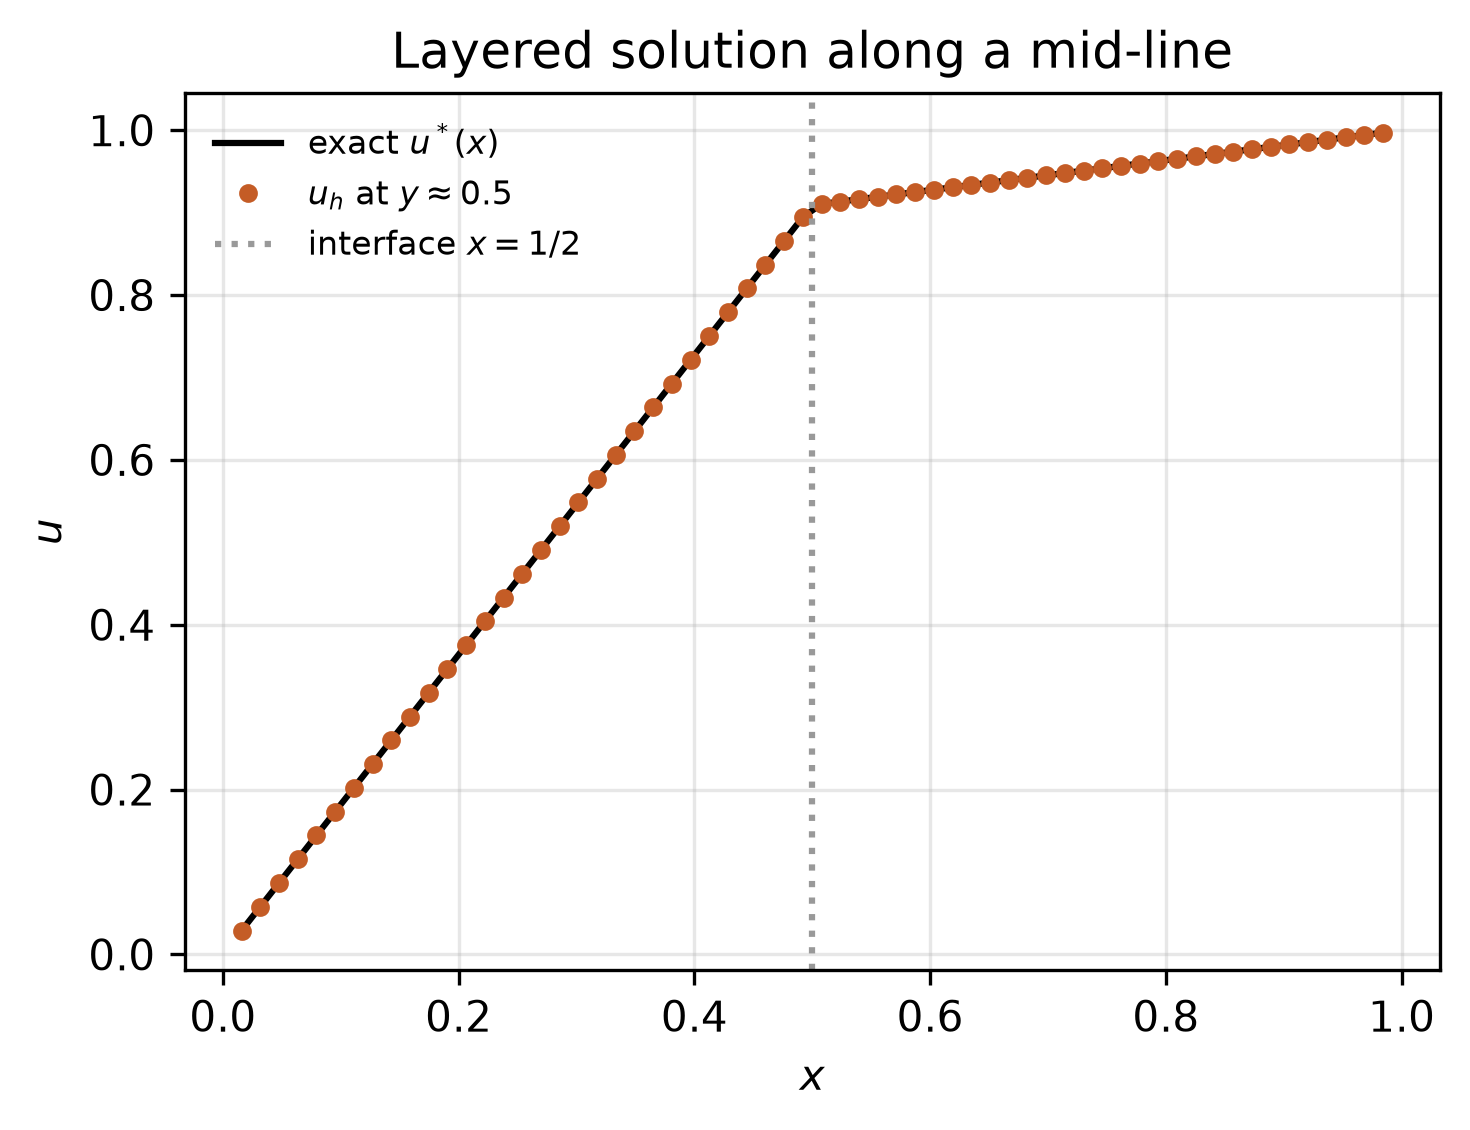
\includegraphics[width=\linewidth]{fig06_layered_profile.png}
  \caption{Profile along \(y\approx 0.5\).}
\end{subfigure}\hfill
\begin{subfigure}[t]{0.48\textwidth}
  \centering
  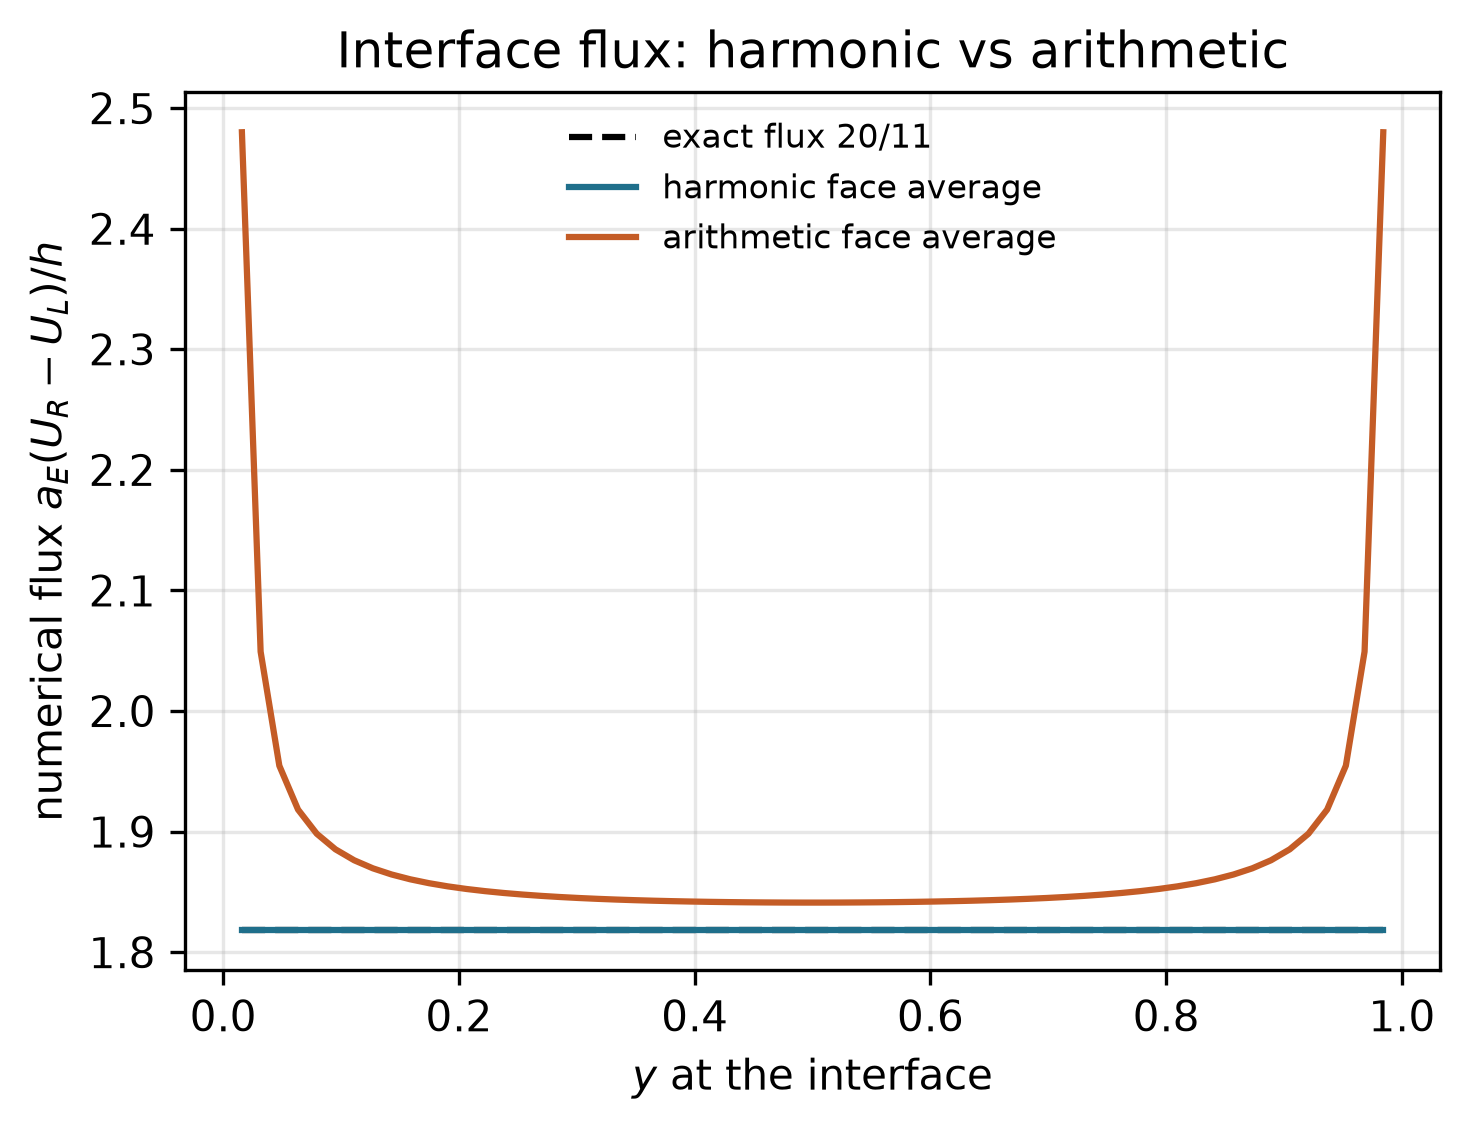
\includegraphics[width=\linewidth]{fig07_layered_flux.png}
  \caption{Interface flux versus \(y\).}
\end{subfigure}
\caption{Left: harmonic \(u_h\) against the exact piecewise-linear profile; the kink at \(x=1/2\) sits between columns. Right: numerical interface flux. Harmonic recovers \(20/11\); arithmetic is a different constant that does not shrink with \(h\).}
\label{fig:profile}
\end{figure}

\begin{figure}[H]
\centering
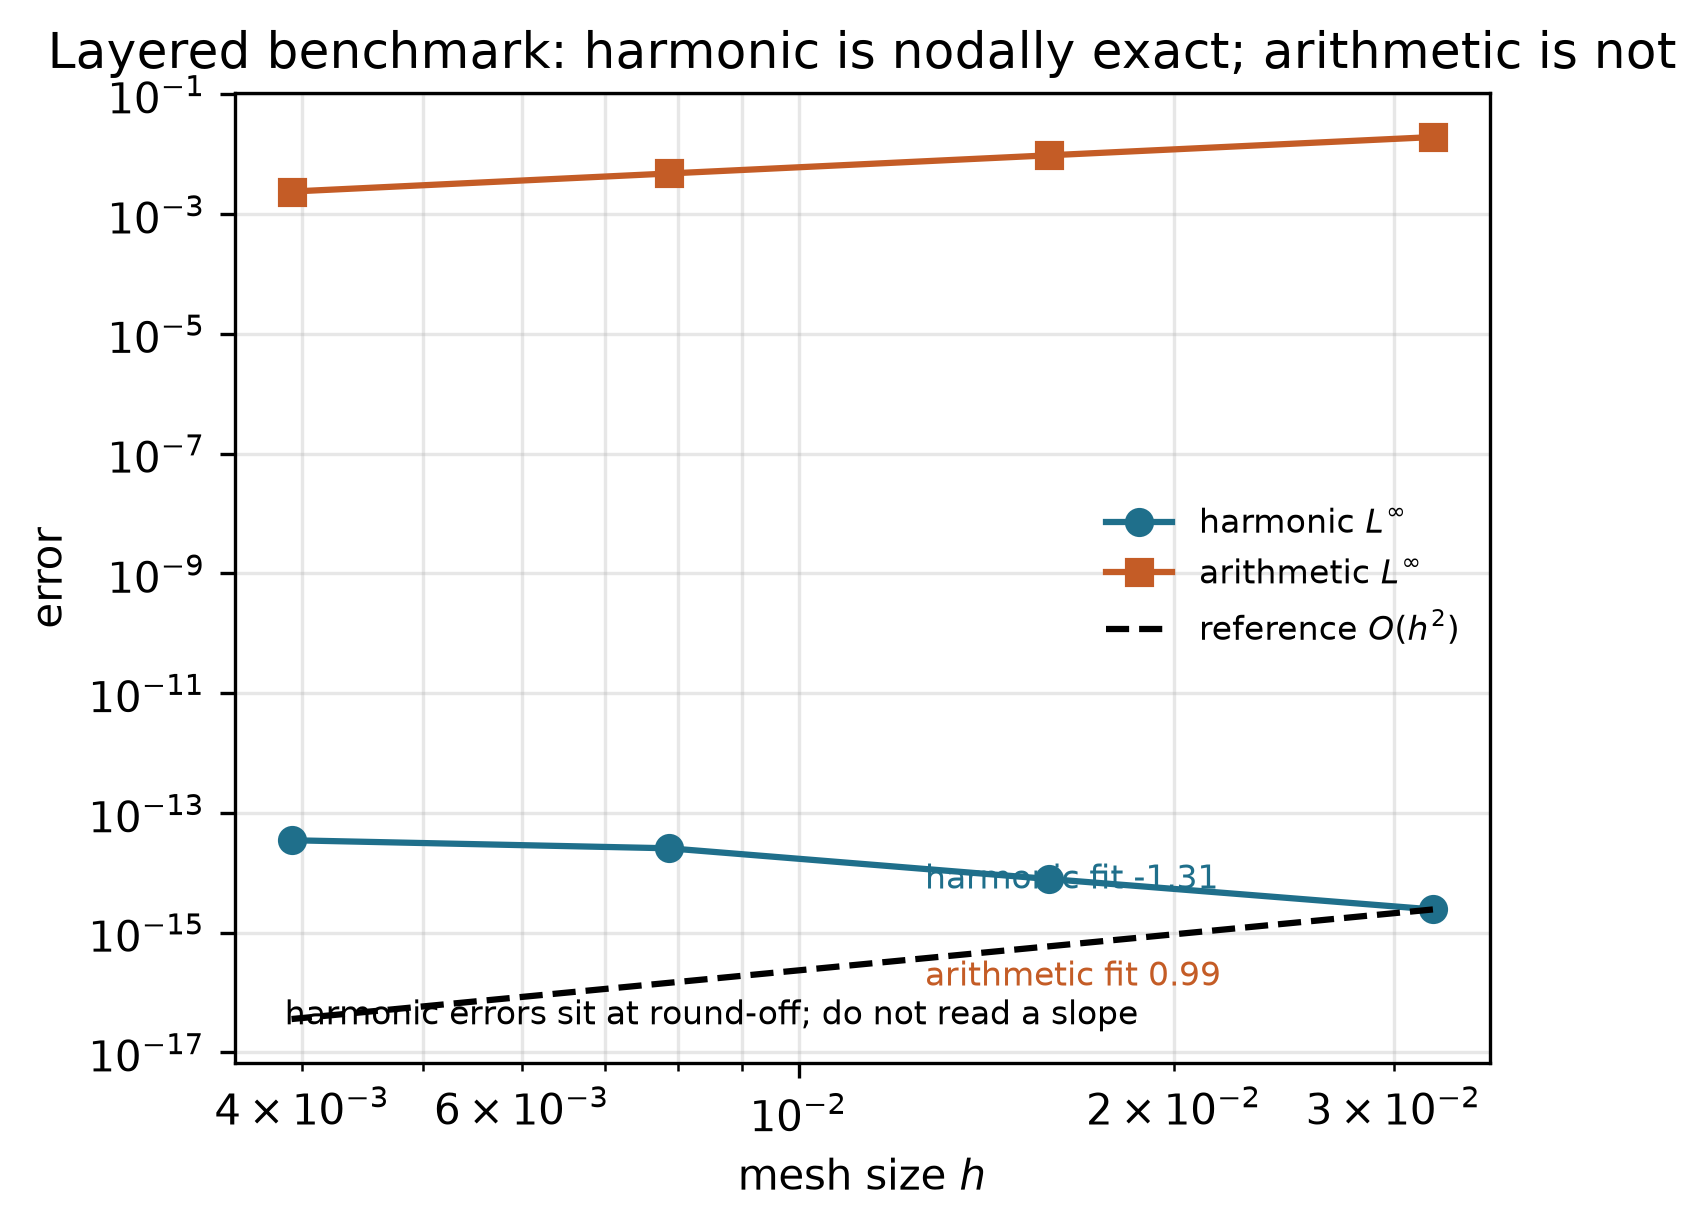
\includegraphics[width=0.62\textwidth]{fig08_order_layered.png}
\caption{Layered \(L^\infty\) versus \(h\). Harmonic errors sit at round-off. Arithmetic tracks first order. Same data, two face rules, named norm: the depth comparison.}
\label{fig:layerorder}
\end{figure}

\subsection{Main Results: Contrast, Conditioning, Cost}
Unpreconditioned CG iteration counts on the layered harmonic matrix at \(n=30\), relative residual \(10^{-10}\), grow with the contrast \(a_R/a_L\): \(125\), \(227\), \(401\), \(615\) iterations at contrasts \(2,10,50,200\) (Figure~\ref{fig:contrast}).
Coefficient contrast worsens conditioning but preserves the discrete maximum principle.
On smooth P4, \(\kappa_2(A_h)\) tracks \(h^{-2}\) as already quoted.

\paragraph{Cost--accuracy at a matched target.}
Cost measure (stated before quoting): CG iteration count to a relative residual, versus one sparse factorisation for \texttt{spsolve}.
Accuracy target (frozen across the comparison): discrete \(L^2\) error equal to the \texttt{spsolve} value \(3.988\times 10^{-4}\) on P4 at \(n=31\).
Not counted: assembly, eigenvalue estimates, figure rendering, and Python interpreter startup.
Table~\ref{tab:cg} and Figure~\ref{fig:cg} (right) show that CG first hits this target at relative residual \(10^{-4}\) (39 iterations, \(\approx 2\,\mathrm{ms}\) wall); \texttt{spsolve} reaches the same \(L^2\) in one factorisation (\(\approx 2\,\mathrm{ms}\)).
Conclusion (negative for CG on this range): at matched discretisation accuracy there is no runtime crossover for \(n\le 31\); unpreconditioned CG only becomes interesting once contrast or mesh size makes factorisation dominate, which is outside the meshes reported here.

\begin{figure}[H]
\centering
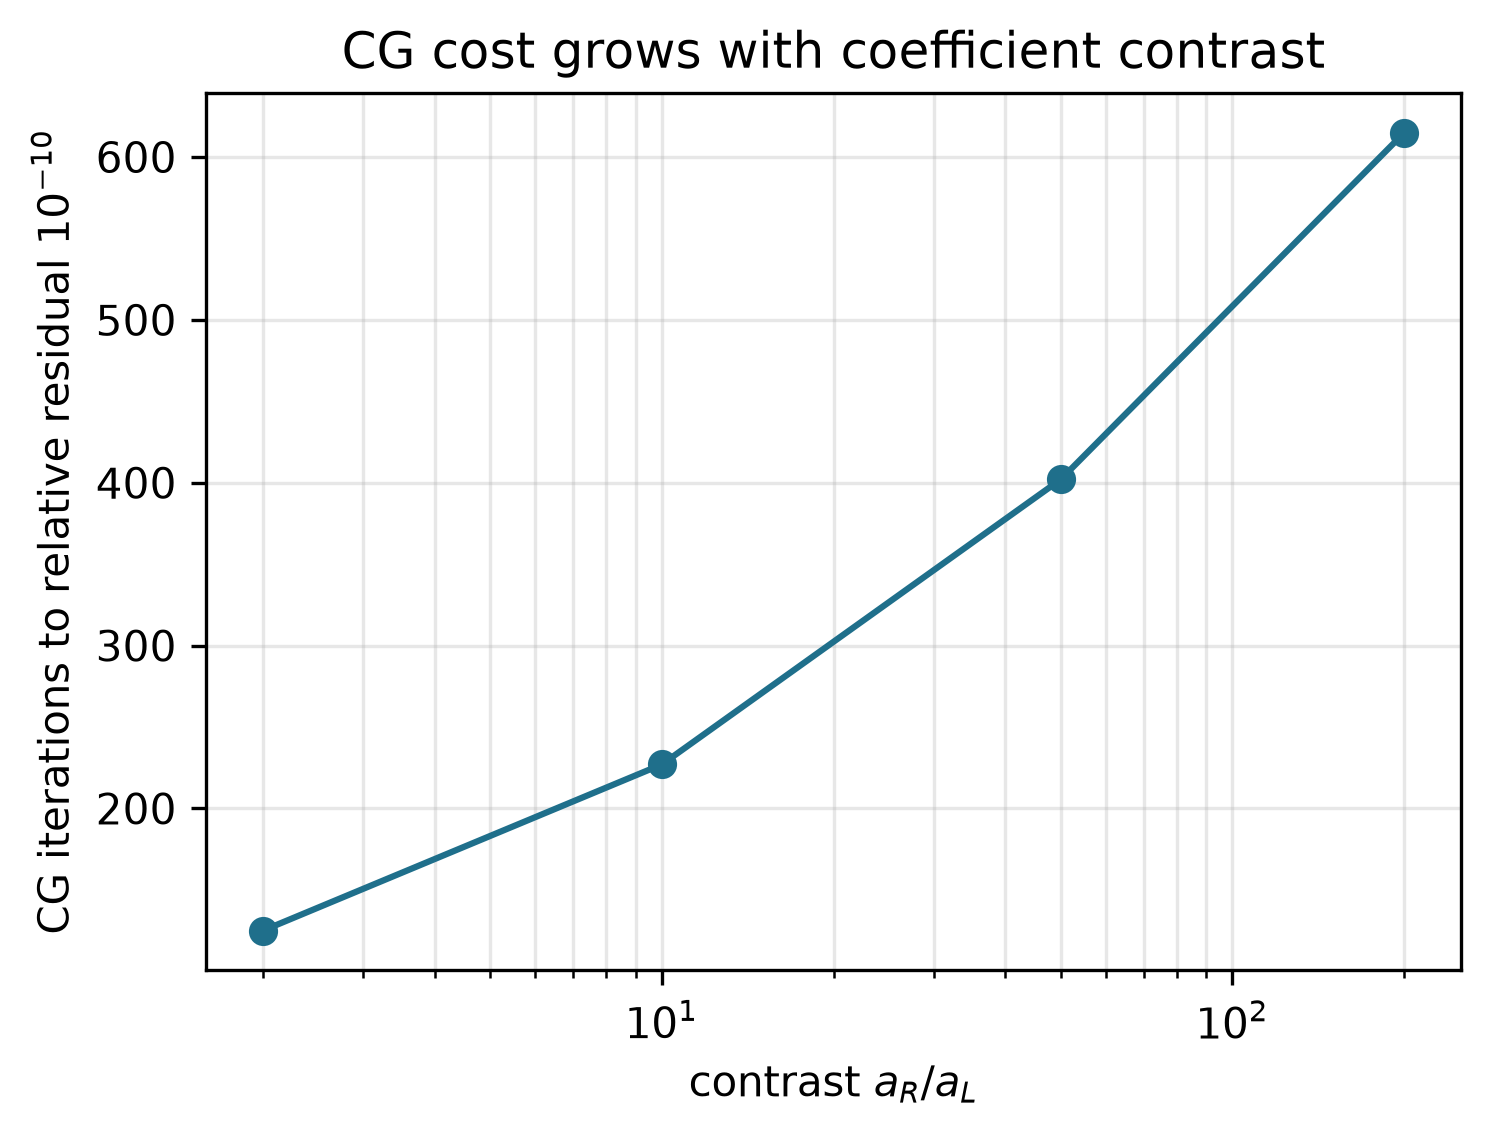
\includegraphics[width=0.62\textwidth]{fig11_iterations_contrast.png}
\caption{CG iterations versus conductivity contrast on the layered problem, \(n=30\), residual stop \(10^{-10}\). Cost measure: iterations. Contrast raises iterative cost without breaking the discrete maximum principle.}
\label{fig:contrast}
\end{figure}

\subsection{Limitations and Robustness}
The second-order claim applies to smooth \(a\) with the half-point face rule.
Across a jump, harmonic averaging on an aligned grid is exact for this piecewise-linear \(u^*\); that is a 1D identity, not a general theorem for rough interfaces that cut cells at arbitrary angles.
Arithmetic averaging remains an M-matrix and still looks smooth on a colour plot, yet its flux is wrong.

I did not implement algebraic multigrid on the FDM matrix, nor a 2D interface-fitted FEM comparison beyond the single P4 oracle.
Unpreconditioned CG will not be competitive on finer 2D meshes; AMG-CG (Tutorial~6) is the natural next solver.
The scheme is Cartesian; a cut-cell disk would need a different boundary row.

\FloatBarrier
\section{Conclusions}
\label{sec:conc}
\begin{itemize}[leftmargin=1.2em]
  \item A conservative face-averaged five-point scheme for \(-\nabla\cdot(a\nabla u)\) with Dirichlet data moved into \(b\) was assembled and verified on the analytic bank before the jump.
  \item On smooth P4, discrete \(L^2\) and \(L^\infty\) both fit order \(2.00\) over four meshes; \(\|A-A^\top\|_{\max}=0\) and \(\lambda_{\min}>0\). The reported rate survives a CG tolerance sweep.
  \item On the layered jump, harmonic face coefficients are nodally exact and keep the flux at \(20/11\); arithmetic coefficients give first-order \(L^\infty\) error and an \(\mathcal{O}(1)\) flux jump. Symmetry is necessary but not sufficient for correct interface physics.
  \item Cost is CG iterations or one sparse factorisation. At \(n=31\), CG and \texttt{spsolve} agree in \(L^2\) once the relative residual is \(10^{-4}\). Next step: AMG-preconditioned CG on finer meshes and non-aligned interfaces.
\end{itemize}

\FloatBarrier
\begin{thebibliography}{12}
\bibitem{hackbusch2017}
W.~Hackbusch, \emph{Elliptic Differential Equations: Theory and Numerical Treatment}, 2nd~ed.\ Berlin: Springer, 2017.
\bibitem{leveque2007}
R.~J. LeVeque, \emph{Finite Difference Methods for Ordinary and Partial Differential Equations}. Philadelphia: SIAM, 2007.
\bibitem{hiptmair2025}
R.~Hiptmair, \emph{Numerical Methods for PDEs}, lecture notes, ETH Z\"urich, 2025.
\bibitem{quarteroni2017}
A.~Quarteroni, \emph{Numerical Models for Differential Problems}, 3rd~ed.\ Cham: Springer, 2017.
\bibitem{scipy2020}
P.~Virtanen et al., ``SciPy 1.0: fundamental algorithms for scientific computing in Python,'' \emph{Nature Methods}, vol.~17, pp.~261--272, 2020.
\bibitem{numpy}
C.~R. Harris et al., ``Array programming with NumPy,'' \emph{Nature}, vol.~585, pp.~357--362, 2020.
\bibitem{skfem}
T.~Gustafsson and G.~D. McBain, ``scikit-fem: a Python package for finite element assembly,'' \emph{Journal of Open Source Software}, vol.~5, no.~52, 2020.
\bibitem{problemPack}
Course problem pack, ``Variable diffusion,'' Project~2 Direction~3, Numerical Analysis of ODEs and PDEs, 2026.
\bibitem{projectBrief}
Course brief, ``Numerical Solution of Elliptic Boundary Value Problems,'' Project~2, 2026.
\end{thebibliography}

\appendix
\section{AI Transparency Log}
\subsection{A1. Tools used}
\begin{center}
\begin{tabular}{@{}llp{0.58\textwidth}@{}}
\toprule
Tool & Date & Primary use\\
\midrule
Cursor (Grok 4.6 agent) & 13--14 Oct 2026 & Week~5 P5 assembly, Dirichlet shift, issue ticket\\
Cursor (Grok 4.6 agent) & 20 Oct 2026 & Week~6 P4 MMS table and log-log slope\\
Cursor (Grok 4.6 agent) & 22 Oct 2026 & Layered harmonic/arithmetic comparison, \texttt{run\_all.py}, report draft\\
\bottomrule
\end{tabular}
\end{center}

\subsection{A2--A3. Claim audits}

\paragraph{Item 1: conservative face stencil and Dirichlet sign.}
\emph{Claim / assumptions:} assemble \(-\nabla\cdot(a\nabla u)\) with \(b_k \mathrel{+}= a_{\mathrm{face}} g/h^2\); boundary nodes absent from \(A_h\).
\emph{Risk / falsifier:} wrong sign on the boundary shift (or treating boundary nodes as unknowns) still produces a smooth-looking \(u_h\).
\emph{Independent check:} P5 centre \(1.651995\) against the bank value \(1.652\) at \(n=15\); P2 \(L^\infty=3.3\times 10^{-16}\); hand matrix \(n=2\) has diagonal \(4/h^2=36\) and \(\mathrm{nnz}=12\) (\texttt{validation\_tests.py}).
\emph{Decision:} keep the interior-only unknown list. \emph{Limitation:} checks cover rectangular Dirichlet problems; Neumann rows were not tested.

\paragraph{Item 2: layered exact profile.}
\emph{Claim / assumptions:} piecewise \(u^*\) continuous with continuous flux \(a u_x\).
\emph{Risk / falsifier:} an OCR'd pack line looked like \(u^*=2x+9/11\) on the right half; that formula is discontinuous at \(x=1/2\) and would falsify every nodal-exact test.
\emph{Independent check:} re-derived \(u^*\) from continuity of \(u\) and of \(a u_x\) with \(u(0)=0\), \(u(1)=1\), obtaining~\eqref{eq:ulayered}. Harmonic FDM then hits \(L^\infty\sim 10^{-14}\).
\emph{Decision:} use~\eqref{eq:ulayered}. \emph{Limitation:} the derivation is 1D; a genuinely 2D jump geometry needs a separate exact solution.

\paragraph{Item 3: arithmetic averaging as ``symmetric, hence correct''.}
\emph{Claim / assumptions:} any consistent positive face average yields a valid interface scheme.
\emph{Risk / falsifier:} reporting \(\|A-A^\top\|=0\) as evidence that the jump is right.
\emph{Independent check:} Table~\ref{tab:layer}---arithmetic is symmetric and monotone, yet the flux jump stays \(0.66\) and \(L^\infty\) is only first order. Harmonic is nodally exact.
\emph{Decision:} quote symmetry as structure; quote flux and nodal error as physics. \emph{Limitation:} the arithmetic case is a deliberate negative control, not a candidate production scheme.

\subsection{A4. Ownership}
I own the stencil derivation, the layered exact profile, the choice of odd-\(N\) grids, the interpretation of arithmetic versus harmonic, and the figures.
AI assistance filled and checked \texttt{assemble.py} / \texttt{run\_all.py} / \texttt{validation\_tests.py} and the first typesetting pass.
Trusted dependencies: \texttt{scipy.sparse.coo\_matrix} and \texttt{spsolve} for the discrete solve; \texttt{scipy.sparse.linalg.cg} with a residual callback; \texttt{eigsh} only as SPD/conditioning corroboration; \texttt{scikit-fem} \texttt{condense}/\texttt{asm} as an optional 2D oracle.
I can explain and modify the FDM assembler without AI during the viva.

\section{Individual Contribution Statement}
\noindent\textbf{Individual Contribution Statement --- Project 2 (PDE BVP)}\\
Name: Chuyang Wang \qquad Student number: 2363591\\
Role this project: sole author (implementation, weekly tasks, report).

The specific things I did this project:
\begin{enumerate}[leftmargin=1.2em]
  \item Derived the conservative stencil~\eqref{eq:stencil} and the Dirichlet shift~\eqref{eq:dirichlet}; implemented them in \texttt{code/assemble.py} with the index map \(k=in+j\).
  \item Completed the Week~5 P5 challenge (\(u_h(0.5,0.5)=1.652\)) and the Week~6 four-mesh slope (\(2.00\) in discrete \(L^2\) and \(L^\infty\)).
  \item Re-derived the layered profile~\eqref{eq:ulayered}, implemented harmonic versus arithmetic face averages, and produced Table~\ref{tab:layer} and Figures~\ref{fig:profile}--\ref{fig:layerorder}.
  \item Separated algebraic from discretisation error by a CG residual sweep (Table~\ref{tab:cg}); measured CG iterations against contrast (Figure~\ref{fig:contrast}).
  \item Wrote \texttt{validation\_tests.py} and \texttt{run\_all.py}, and wrote the full \LaTeX\ report including the AI log and this ICS.
\end{enumerate}
What I would do differently: freeze the layered exact formula on paper before reading the OCR'd pack, instead of debugging a ``failed'' nodal-exact test against a discontinuous \(u^*\).\\
Anything I should have asked for help with earlier: whether odd \(N\) (interface between columns) versus even \(N\) (interface on a node) is required for the FDM sanity check, before running the first layered table on \(n=15\).\\
Signature: \underline{\hspace{4cm}} \quad Date: \underline{\hspace{3cm}}

\section{Supplementary data}
P4 structure at \(n=15\): \(\|A-A^\top\|_{\max}/\|A\|_{\max}=0\), \(\lambda_{\min}=28.61\), \(\kappa_2\approx 1.27\times 10^{2}\).\\
FEM 1D element matrix for \(h=1/4\): \(\bigl(\begin{smallmatrix}4&-4\\-4&4\end{smallmatrix}\bigr)\).\\
All numbers in the tables are reproduced by \texttt{python code/run\_all.py}.

\end{document}
